
%----------------------------------------------------------------------------
\chapter{Preliminaries}
%----------------------------------------------------------------------------

In this chapter We revisit the background knowledge on graph-based modeling, and graph pattern matching. We also introduce the used terminology as it is crucial in the following chapters. At the end of the chapter we show how the concepts of graph pattern matching can be extended for distributed systems.

\section{Graph-based modeling}

Structural and behavioral modeling of systems are often done using graphs. 
Graphs are useful as they are easy to understand, intuitive to use, and lots of existing algorithms can be used to process them. 
As the model-based approach used by the framework uses models of graph based formalism, in this section, graph-based modeling is presented.

A directed graph consists of a set of nodes and a set of edges, where edges are a tuple of two node: its \emph{source} node and its \emph{target} node. 
Graphs can be extended to make them suitable for modeling:

\begin{itemize}
	\item by each node having a type
	\item by each edge having a type implying its semantics and restricting what type of nodes can they connect
	\item by nodes having attributes with given values (e.g.\ name)
\end{itemize}


\begin{figure}[H]
	\begin{center}
		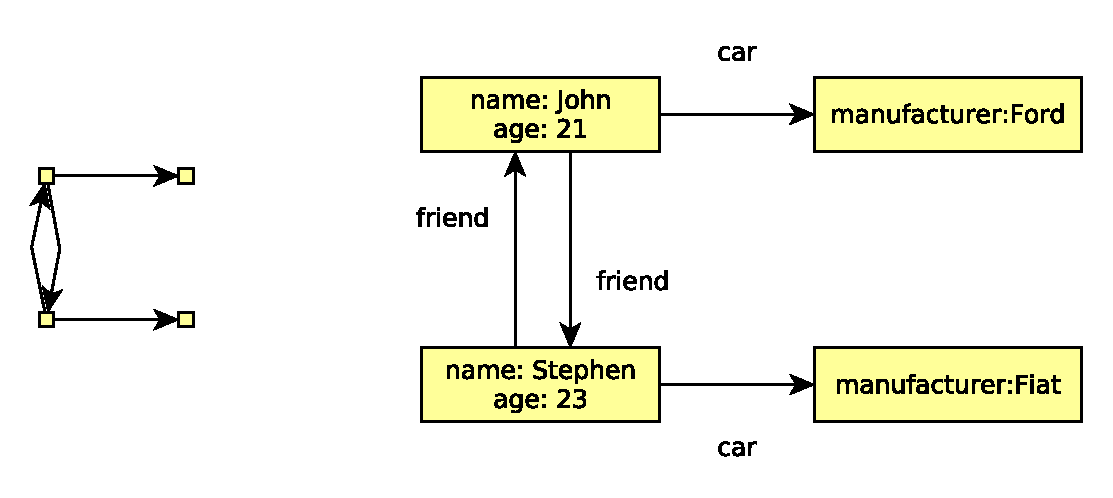
\includegraphics[width=\textwidth]{figures/graphs.pdf}
		\caption{Basic graph (left), and extended (right) }
		\label{fig:graphs}
	\end{center}
\end{figure}

In case of this extended graph model we also use the term \emph{object} for a typed node with attributes and \emph{reference} for a typed edge. This is consistent with the terminology used in software engineering.

With this extended graph model, there is also a need to give rules for certain types of models, which is the role of \emph{meta modeling}.
A meta model is a model, that defines how the graph model of a system is built up:
\begin{itemize}
	\item what type of objects are exists
	\item what kind of attributes can a node of a certain type has (name and type)
	\item what type of references exist and what type of object can be its source and target node
	\item multiplicity restriction for references and attributes
	\item hierarchical relationship between types
\end{itemize}

\autoref{fig:metamodel} show some of these concepts. The upper part is a meta model, and the lower is an instance model, that satisfies the rules defined by the metamodel: There can be 3 type of object: \texttt{ModelElement}, \texttt{Train} and \texttt{RailRoadElement}. All instance of \texttt{ModelElement} has an id. Both of \texttt{Train} and \texttt{RailRodeElement} are a subtype of \texttt{ModelElement} which means, that each instance of the subtype works as an instance of the supertype too.
\begin{figure}[h]
	\begin{center}
		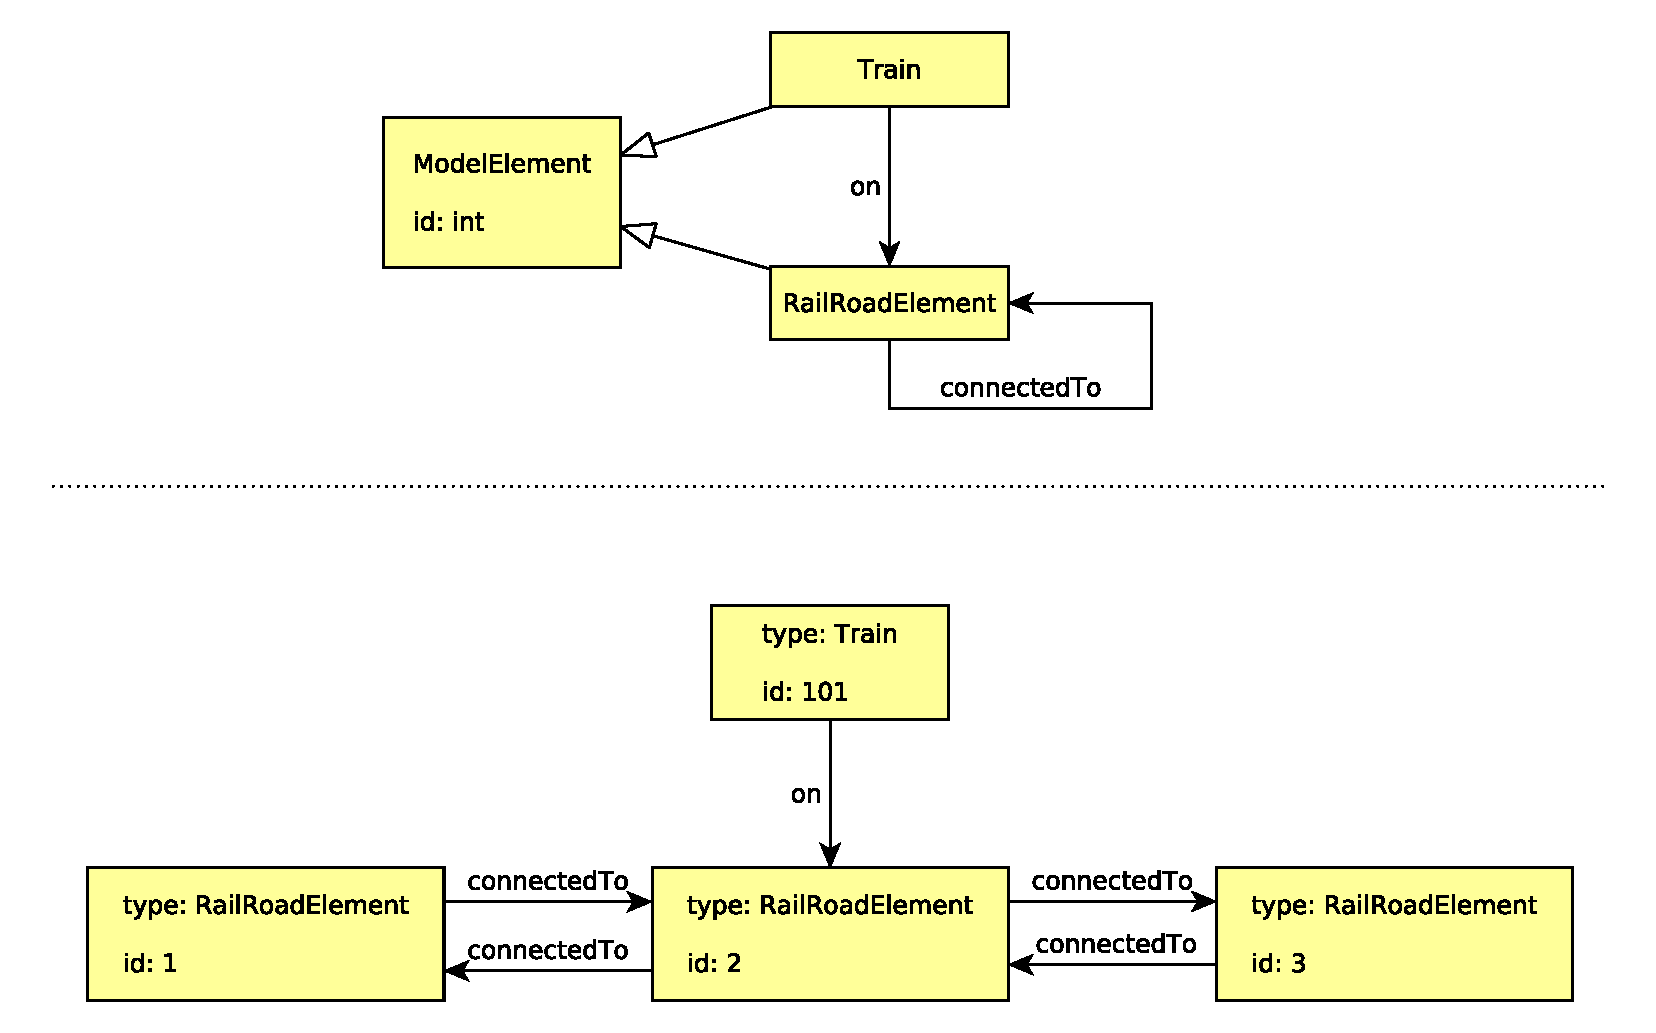
\includegraphics[width=\textwidth]{figures/metamodel.pdf}
		\caption{ Example of a meta model and an instance model }
		\label{fig:metamodel}
	\end{center}
\end{figure}


\section{Domain and runtime modeling}

In this framework, we use graph-based models to represent the current state of the system. 
The state and the operating context of the system is captured in a model called the \emph{live model} or \emph{runtime model}.
It is updated with sensor data and information from other sources, so the model represents the physical system's latest state.
An example for this is depicted on \autoref{fig:live-models}. As train 105 is moving to a new segment of railway, sensors watching its position send updates to the model, which is getting modified to represent, that the train is now on a new segment.


This model is used for runtime verification.
While the model is being continuously updated it is also analyzed using graph pattern matching to find parts of the model that may imply.


\begin{figure}[H]
	\begin{center}
		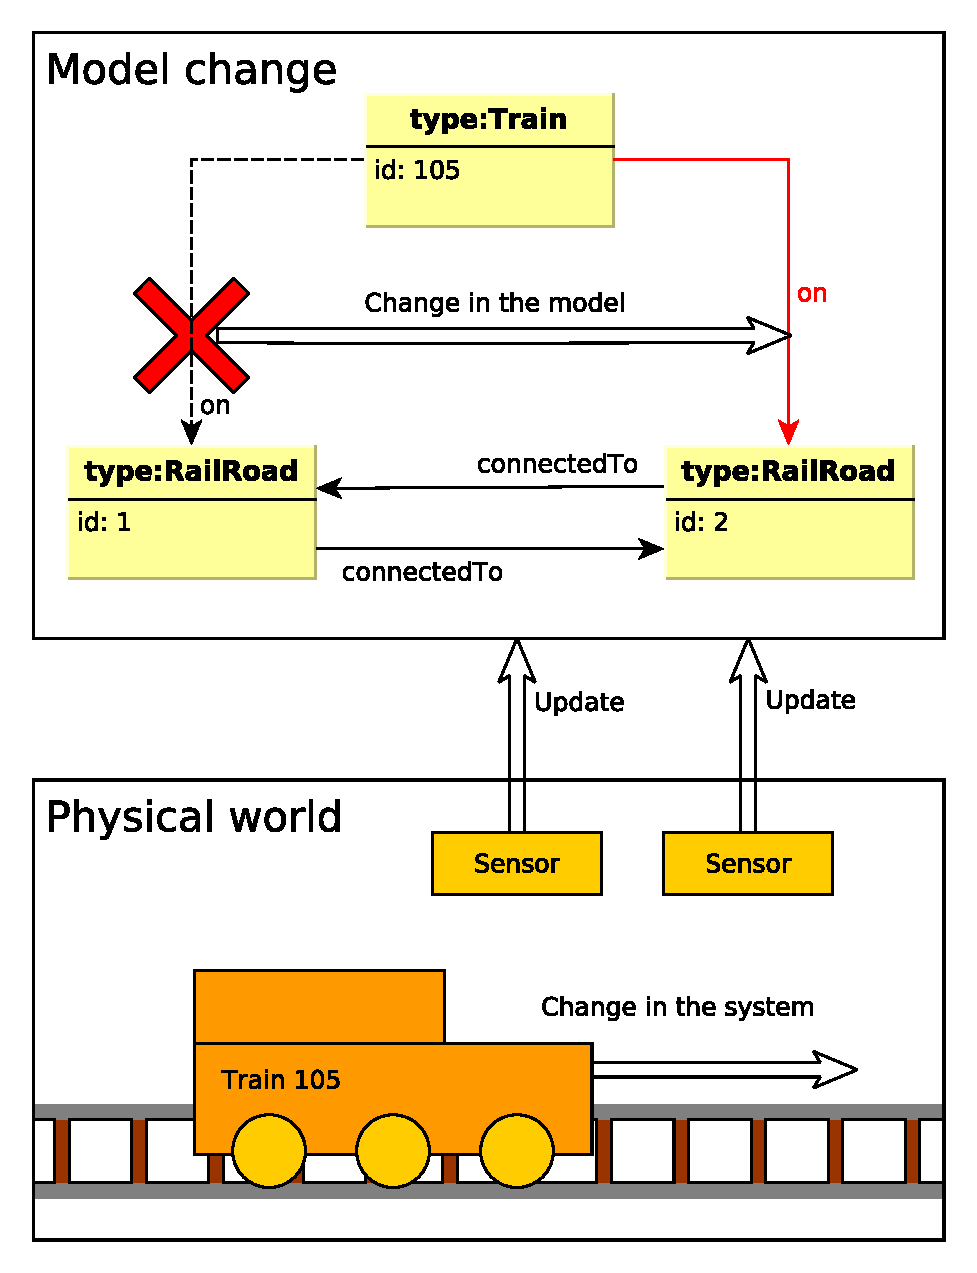
\includegraphics[width=0.7\textwidth]{figures/live-models.pdf}
		\caption{Live model updating}
		\label{fig:live-models}
	\end{center}
\end{figure}

\section{Foundations of graph pattern matching}
\label{section:gpmc}

\todo{Marci tanácsait bevezetni, ha frissebb leszek}
\todo{Tetszőleges kifejezéssel lehet gráf patternt adni, viszont a viatra és a local search miatt adott egy értelmes formához kötni magunkat}

The goal of graph pattern matching is to find all the subgraphs of a graph meeting a certain criteria, defined by a \emph{graph pattern}.

Let's define the domain of an extended graph as the union of 
\begin{itemize}
	\item the set of the vertices of the graph
	\item and the set of data values (Strings, numbers, boolean values, and enumeration literals), which from its attributes can take their values
\end{itemize}

Then a \emph{graph pattern} is a predicate, which's domain is the domain of the extended graph.
A \emph{pattern match} is a tuple, that satisfies the predicate.
A pattern's \emph{matchset} is the truth set of the predicate, i.e.\ the set of tuples that satisfies the predicate.
A \emph{graph query} is a program or execution plan capable of calculating the matchset of a graph pattern on a given graph. 



We build up graph patterns with a modified\footnote{ Absence of universal quantification and functions of terms.  } first-order logical formula the following way:
\begin{itemize}
	\item Terms can be variables and constants, constants only refer to data values.
	\item Constraints are a predicate applied to terms. 
	\item A formula can be a constraint, or an expression composed of logical connectives (and, or) and existential quantifier ($\exists{}$) used with other formula.
	\item The graph pattern itself is a formula.
\end{itemize}

We use the following constraints as basic elements of a graph patterns:

\begin{itemize}
	\item Type constraint -- Satisfied, when the variable's value is a vertex of a given type
	\newline Type(Variable)
	
	\item Reference -- Satisfied, when an edge with a given label exists from the first variables value to the second variables value (vertex only)
	\newline ReferenceName(Source variable, Target variable)
	
	
	\item Attribute -- Satisfied, when a variable has a given attribute being the same as the other variables value (data only)
	\newline AttributeName(variable, attribute value)
		
	\item Equality -- two variable's values are the same
	\newline var1 = var2
		
	\item Inequality -- two variable's values are different
	\newline var1 $\neq$ var2
	
	\item Pattern match -- a tuple of variable values are a match of another pattern	
	\newline PatternName(v1, v2, \dots{}).
	
	\item Negative pattern match -- a tuple of variable values are not a match of another pattern	
	\newline PatternName(v1, v2, \dots{}).
	
	\item Pattern count -- Counts the matches of a pattern.
	\newline $v_{out} = \text{count PatternName}(v1, v2, \dots{})$.
\end{itemize}

We can also use a visual representation (see Fig. \ref{fig:pattern-visual}) to illustrate a graph pattern, altough textual languages (see VQL) is used in the framework.

\begin{figure}[h]
	\begin{center}
		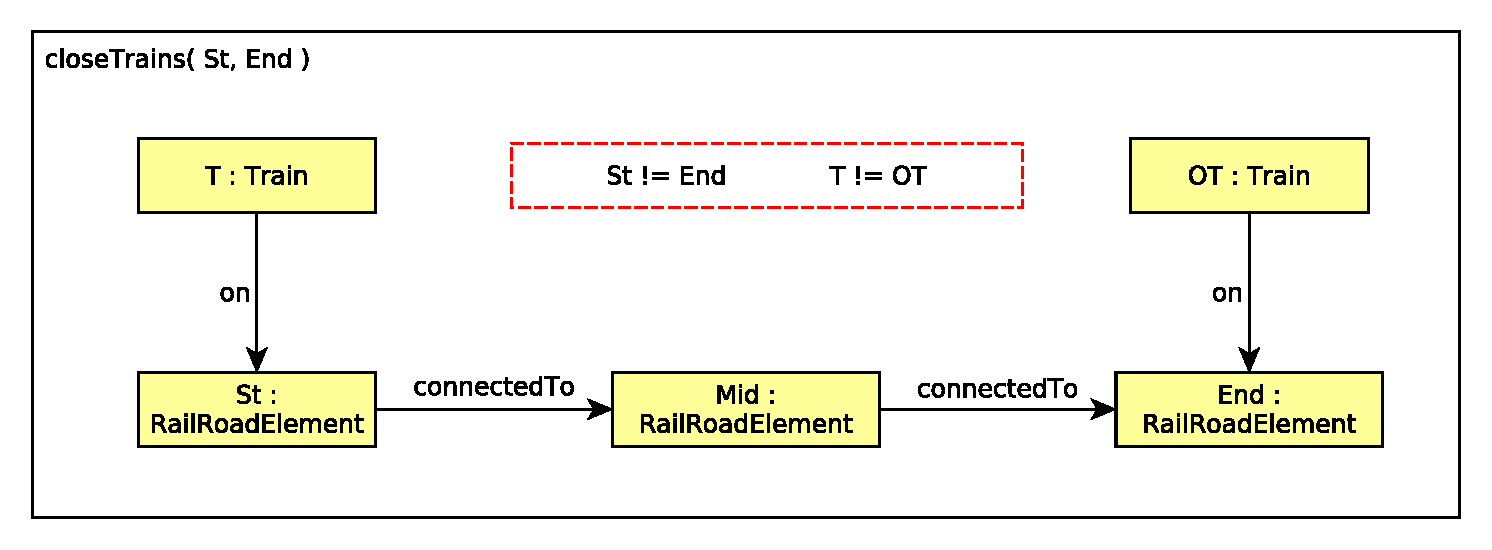
\includegraphics[width=\textwidth]{figures/closeTrains-pattern.pdf}
		\caption{Visual representation of a graph pattern}
		\label{fig:pattern-visual}
	\end{center}
\end{figure}


\section{Local search-based graph pattern matching}
\todo{Ide is bevezetni marci kommentjeit}


Local search refers to a family of algorithms solving problems involving a search space. 
Local search starts from a candidate solution for a problem, then searches by applying local changes: moving to neighboring locations until solutions are found.

Local search can also be used to provide a matchset for a graph pattern in a graph.
It is also a memory-efficient alternative for rete algorithm in \viatra{}~\cite{bur-marton-msc}.

In our system we use local search-based graph pattern matching. 
Let's assume, that a graph pattern is given as a conjunction of expressions (bodies) that existentially quantifies the variables, then checks if the constraints are met.
We can do this, by outsourcing negated expressions to subpatterns and use negative pattern match constraint, and using other transformations.
As VQL permits this structure only, the framework does not do these transformations.


\begin{equation}
\begin{array}{@{}r@{}l@{}l@{}l@{}l@{}l@{}}
Pattern(p1, p2, \dots) = \;
& \exists{x_1} & \exists{x_2}... \: & 
(Constr_{11}(\bar{p},\bar{x} ) & \, \wedge \, Constr_{12}(\bar{p},\bar{x} ) & \, \wedge \, \dots{}) \: \vee \\

& \exists{y_1} & \exists{y_2}... \: & 
(Constr_{21}(\bar{p},\bar{y} ) & \, \wedge \, Constr_{22}(\bar{p},\bar{y} ) & \, \wedge \, \dots{}) \: \vee \\
& \dots{}
\end{array}
\end{equation}

We use the term body to denote a line of a pattern structured this way.
We can find the truth set of this expression, by finding the truth sets of all the bodies as distinct predicates on the parameters, and taking their union.
Our problem now is the following: find all the variable bindings, which satisfies the constraints of the body.

The algorithm is the following:



\todo{ez itt finomítható}

The search space consists of all the possible variable bindings (leaving a variable unbind is also a possibility). 
We start from all variable being unbound. 
We go through the constraints and with each constraint, we do one of the following:
\begin{itemize}
	\item Check operation: If all the variables referred by the constraint are bound, then we check if they satisfy the constraint. If yes, we follow the algorithm, if not we backtrack.
	\item Extend operation: If a variable is unbound then we iterate through all the possible values that satisfies the constraint, and for each value we bind it to the variable and follow the algorithm. After all the possible values are done, we backtrack.
\end{itemize}

This structure leads to a search tree.
It can be easily proved, that at the $i$th layer of the tree, the first $i$ constraint is satisfied, as a child node not modifies already bound variables.
This means, that after the last constraint, the variable binding satisfies all the constraints, so it can be projected to the variables to find a solution.
It can also be proved, that all of the variable bindings satisfying the constraints can be found: 
consider this variable bindings, and call this the goal binding. Now start the algorithm: each extend operation can bind the unbound variables as in the goal binding, and each check operation will find the constraint satisfied for the variable binding.

We use depth first search, because it uses less memory, and it can be easily used to synthesize code, as the layers are well defined. This way search can be easily implemented using nested for loops.


\section{Distributed computational platform}

% adatok diszjunkt halmazokra bontva különböző csomópontra
% az algoritmusok is elosztottak, nem lesz összegyűjtve az infó, úgy van kiértékelve, hogy nincs aki mindent látna a rendszerből

As cyber-physical systems are distributed we must deal with the sensor data coming from different sensors at different computation units of the system because of the locality of data. 
Sending the sensor data to one computation unit and evaluate on that can cause different problems: 
sensor data can be too large to be sent over network, the central node can be a SPOF~(Single Point of Failure), etc. 

In the presented framework the live model is distributed on the different computation units and the graph pattern matching algorithm itself runs in a distributed way. 
This eliminates the problem of central computers, but introduces complexity, that we must handle.
One of the problems is distributed model handling, and the other is how to execute queries efficiently on a distributed platform.





\subsection{Distributed graph models}

In this thesis, the phrase \emph{computing unit} is used to denote a physical or virtual execution component of the cps that is capable of storing a part of the graph model and updates it to fit the current state the physical world, eg.\ an embedded system or a virtual machine.

In our framework each node in the graph is allocated to a computing element. 
On that computing element, that node is called a \emph{local node}. 
In the context of other computing modules it is called a \emph{remote node}. 
Edges are stored in the computing module of their source node; 
If their target node is not a local node on that node, a \emph{proxy node} is used to substitute the remote node.



\begin{figure}[h]
	\begin{center}
		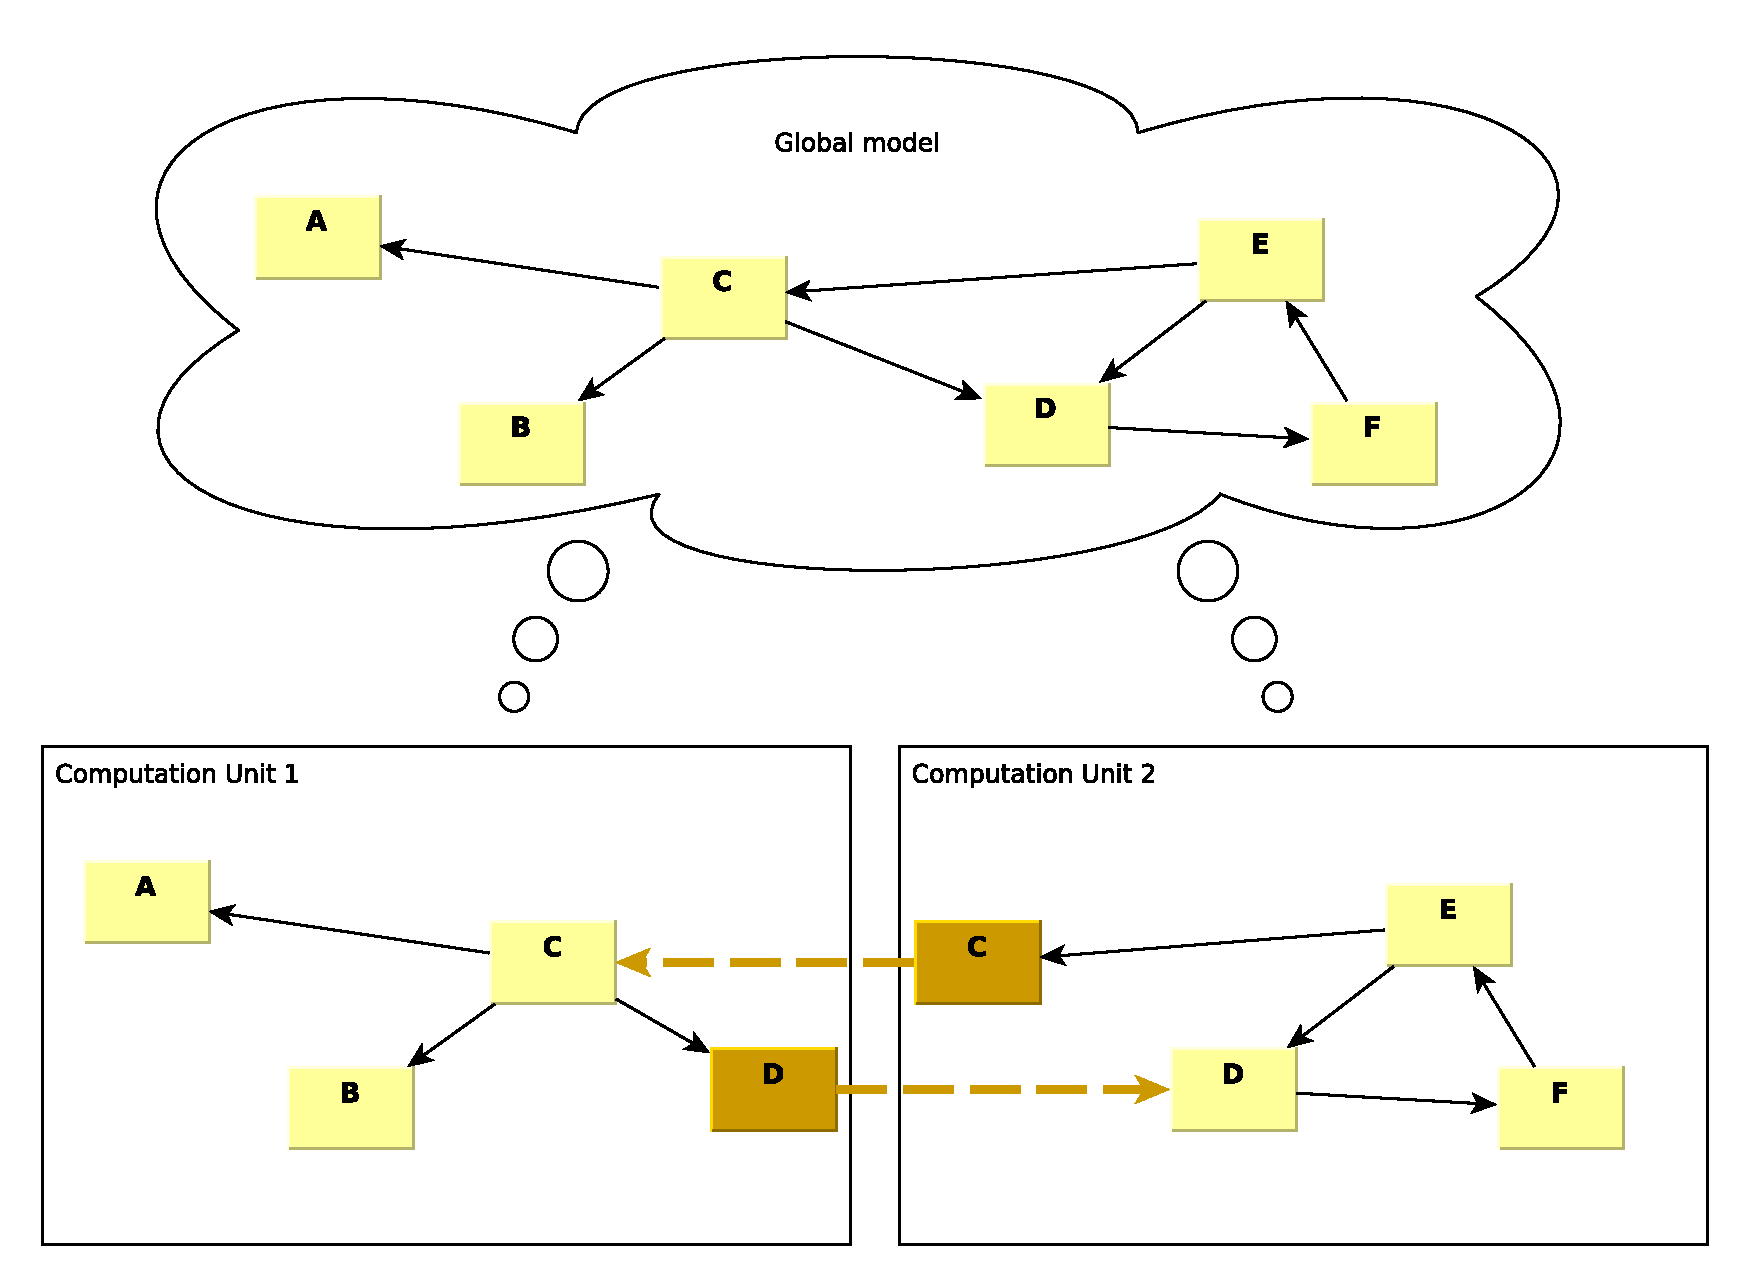
\includegraphics[width=\textwidth]{figures/distributed-model-handling.pdf}
		\caption{Handling distributed models and cross-references}
		\label{fig:distributed-model-handling}
	\end{center}
\end{figure}



\subsection{Distributed query execution}

Distributed query execution is used in the framework to provide matches to graph patterns.
The purpose of distributed query execution is to run queries on distributed models on multiple computers. 
This introduces complexity, as we need to minimize network load, find matches, that can span over multiple model parts, and provide low response times, despite the distributed structure of the model.


\begin{figure}[h]
	\begin{center}
		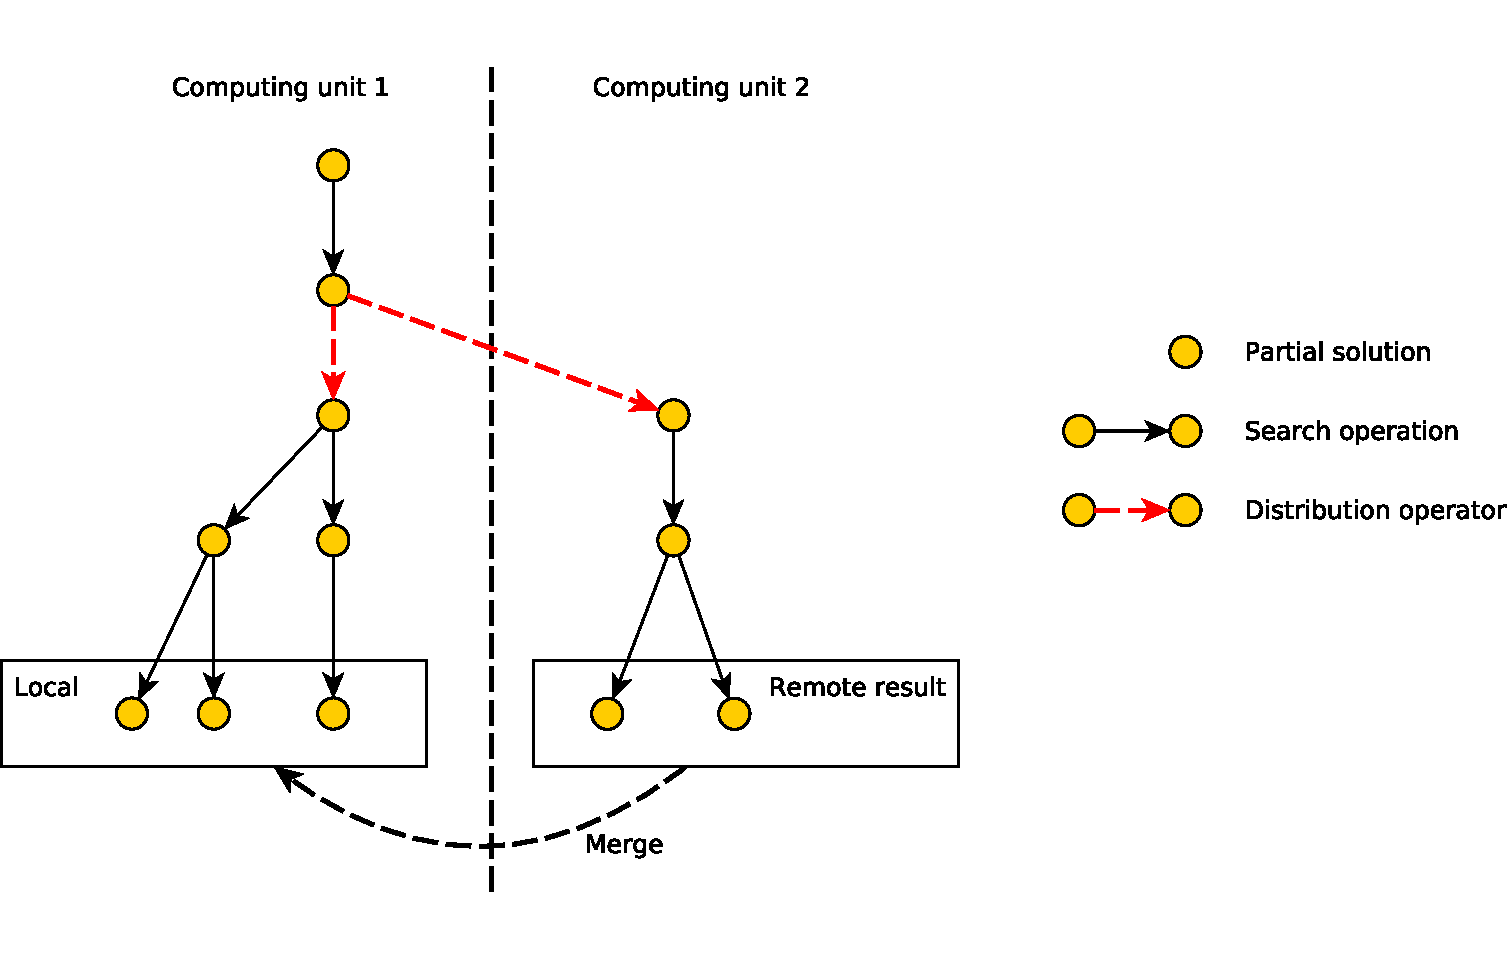
\includegraphics[width=\textwidth]{figures/distributed-ls.pdf}
		\caption{Distributed localsearch operation}
		\label{fig:distributed-ls}
	\end{center}
\end{figure}

In the framework, we extended local search-based graph pattern matching to work on distributed models.
This is achieved by doing the basic search operations locally, but create additional operations, which works in a distributed manner. 
Their mechanism is depicted on \autoref{fig:distributed-ls}.
These operations transmits the query execution to other computing units.
Those units continues to execute the query locally, and when their results are calculated, they send it back to the caller.
The caller waits for the results, and merges the local and remote results.

In this framework, we introduce two distributed operations:
\begin{itemize}
	\item Global distribution: globally distributes the query execution to all computing units (broadcast mechanics).
	\item Aimed distribution, distributes the query execution to the node, which contains a given model element.
\end{itemize}

The first can be used, to globally iterate throw all elements of a given type. The latter is to help navigation through references, as references are stored locally.





